\documentclass[10pt,aspectratio=43,mathserif]{beamer}		
% Beamer, 10pt,4:3, mathserif

\mode<presentation>

\usepackage{NUSTM}
% \usepackage[UTF8]{ctex}    % CN version
\usepackage{xeCJK}
\usepackage{amsmath,amsfonts,amssymb,amsthm,bm}
\usepackage{color}
\usepackage{graphicx,hyperref,url}
\usepackage{times}
\usepackage{verbatim}
\usepackage[square, numbers]{natbib}
\setbeamertemplate{bibliography item}[text]

% \pgfplotsset{compat=1.17}
%%%%%%%%%%%%%%%%%%

\setsansfont{Times New Roman}


% Beamer theme
\beamertemplateballitem


\AtBeginSection[]
{
  \begin{frame}<beamer>
    \frametitle{\textbf{Contents}}
    \textbf{\tableofcontents[currentsection]}
  \end{frame}
}


%%%%----Title settings----%%%%
\title[季度总结]{\fontsize{13pt}{18pt}\selectfont {2021第二季度总结}}
% \subtitle{\fontsize{9pt}{14pt}\selectfont \textbf{利用公共网关的SMS生态系统的安全性描述}}			
%%%%----Title settings


% \author[R. Song]{
%   Bradley Reaves, Nolen Scaife, Dave Tian, Logan Blue, \\
%   Patrick Traynor and Kevin R.B. Butler \\\medskip
%   {\small {\{reaves, scaife, daveti, bluel\}@ufl.edu}} \\
%   {\small {\{traynor, butler\}@cise.ufl.edu}}}
\author[X.Q. Shen]{
Xiangqing Shen\\
{\small {xiangqing.shen@njust.edu.cn}}}
%%%%----Personal info

\institute[NUSTM]{
  Text Mining Lab (NUSTM)\\
  Nanjing University of Science and Technology}
%%%%----Institute Info

\date[\today]{
 \today}
%%%%----Date


\begin{document}

\begin{frame}
\titlepage
\end{frame}				% Title page



\section*{Contents}

		\begin{frame}
		\frametitle{\textbf{Contents}}
		\textbf{\tableofcontents}
		\end{frame}				% Content Page

\section[总结]{工作总结}

		\begin{frame}
			\frametitle{\textbf{工作情况}}
            \begin{block}{\textbf{上季度计划}}
                \begin{itemize}
                    \item 进行事件抽取任务的文献调研,文献阅读的入门工作
                \end{itemize}
            \end{block}

            \begin{block}{\textbf{计划主要完成情况(按时间顺序)}}
                \begin{itemize}
                    \item 季度初做了一个较系统全面的知识图谱Slides并做了组会报告
                    \item 阅读事件抽取相关资料(博客,Slides)、相关论文(7篇),收集相关数据集(2个)
                    \item 完成三门课的课程作业,包括论文复现(1个)、论文翻译(1篇)、小论文(1篇)和相关实验报告(4份)
                    \item 期间转换方向重点,阅读李忠阳大论文(1篇)、小论文(6篇)和其他事理图谱相关论文(7篇)
                    \item 其他穿插任务:Few-shot Learning综述(1篇)、深度强化学习书籍(1部)、变分推断……
                \end{itemize}
            \end{block}
        \end{frame}


\section[细节]{工作内容细节展示}

		\begin{frame}
		  \frametitle{\textbf{知识图谱组会报告(第1周)}}
            \begin{figure}[!t]
            \centering
            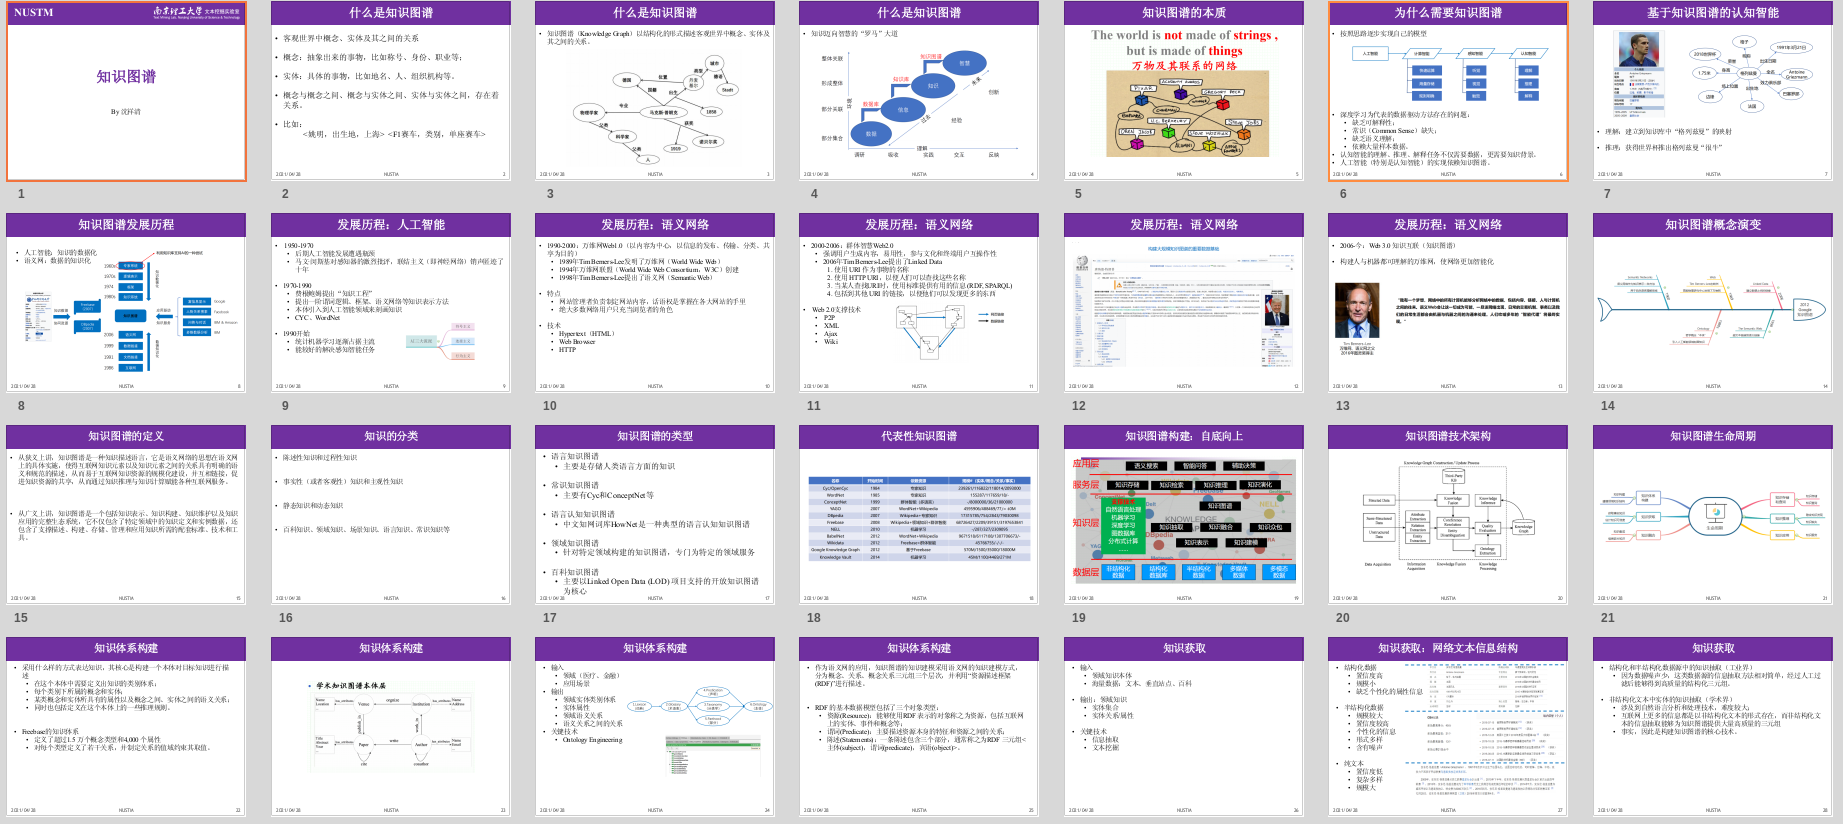
\includegraphics[width=4in]{figures/kg.png}
            \caption{知识图谱Slides}
            \label{fig:kg}
            \end{figure}
            \centering 一个较为系统全面的知识图谱的专题报告。
		\end{frame}

		\begin{frame}
		  \frametitle{\textbf{事件抽取调研和入门(第2-5周)}}
            \begin{figure}[!t]
            \centering
            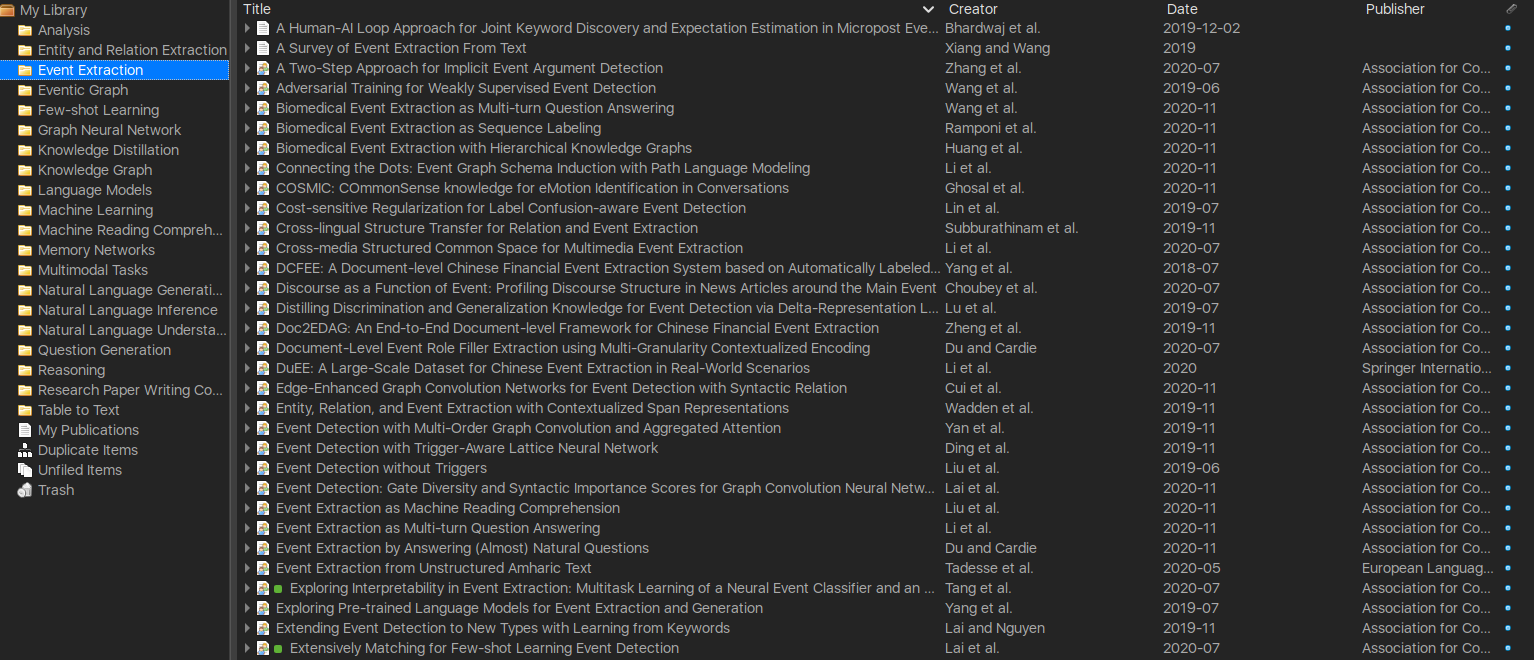
\includegraphics[width=4in]{figures/ee_papers.png}
            \caption{本地维护的事件抽取论文列表}
            \label{fig:ee}
            \end{figure}
            收集的常用数据集为ACE2005、BioNLP等;博客、Slides等略。
		\end{frame}

        \begin{frame}
		  \frametitle{\textbf{模式识别课程作业(第3-4周)}}
			\begin{figure}[!t]
            \centering
            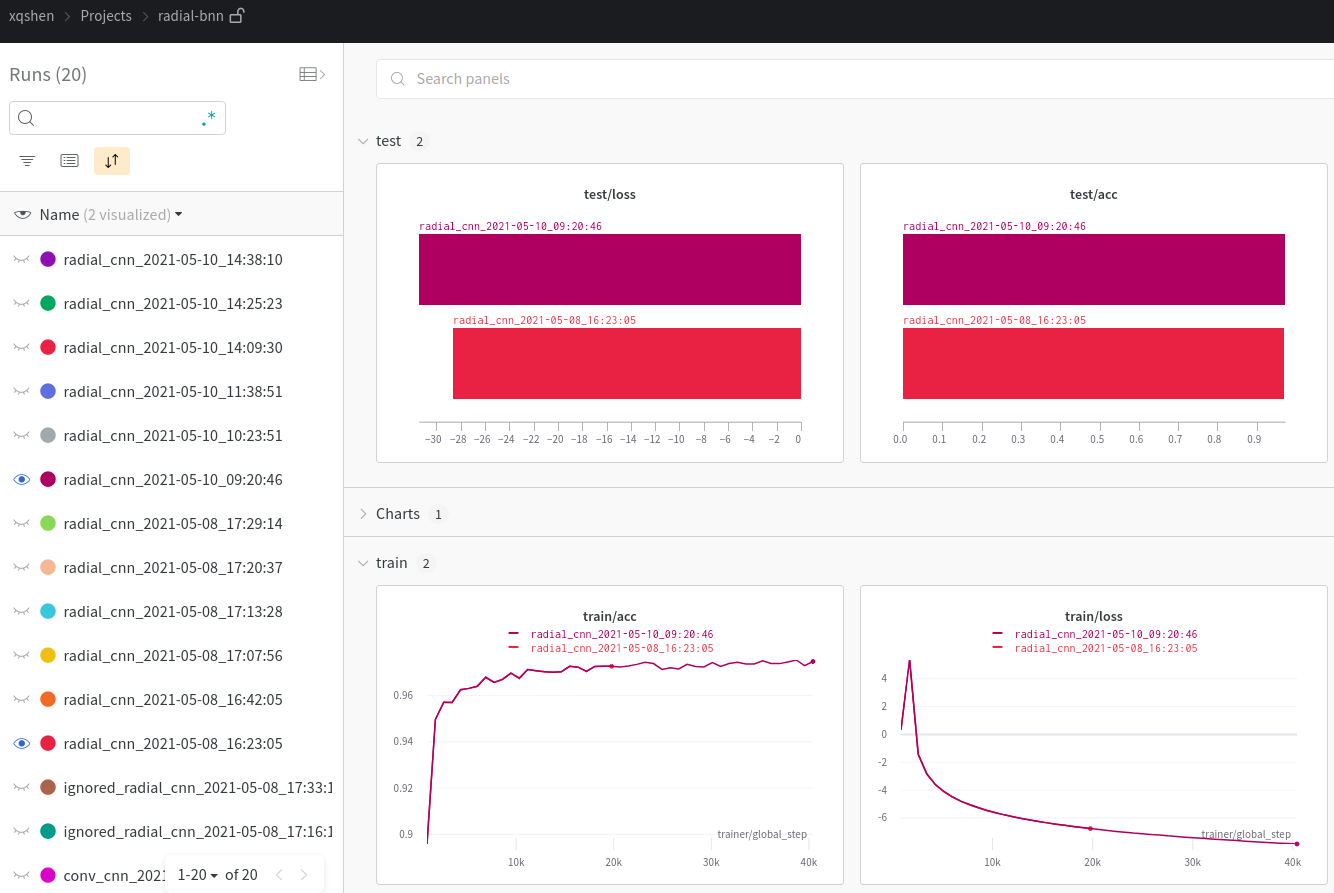
\includegraphics[width=3in]{figures/pr.png}
            \caption{模式识别课程作业}
            \label{fig:pr}
            \end{figure}
            \centering \small {代码:\href{https://github.com/RomanShen/radial-bnn}{https://github.com/RomanShen/radial-bnn}\\
            结果:\href{https://wandb.ai/xqshen/radial-bnn?workspace=user-xqshen}{https://wandb.ai/xqshen/radial-bnn?workspace=user-xqshen}}
		\end{frame}

        \begin{frame}
		  \frametitle{\textbf{FSL、RL、VI、\LaTeX(第4-7周)}}
            \begin{columns}[b]

                \column{.26\textwidth}
                \begin{figure}
                    \centering
                    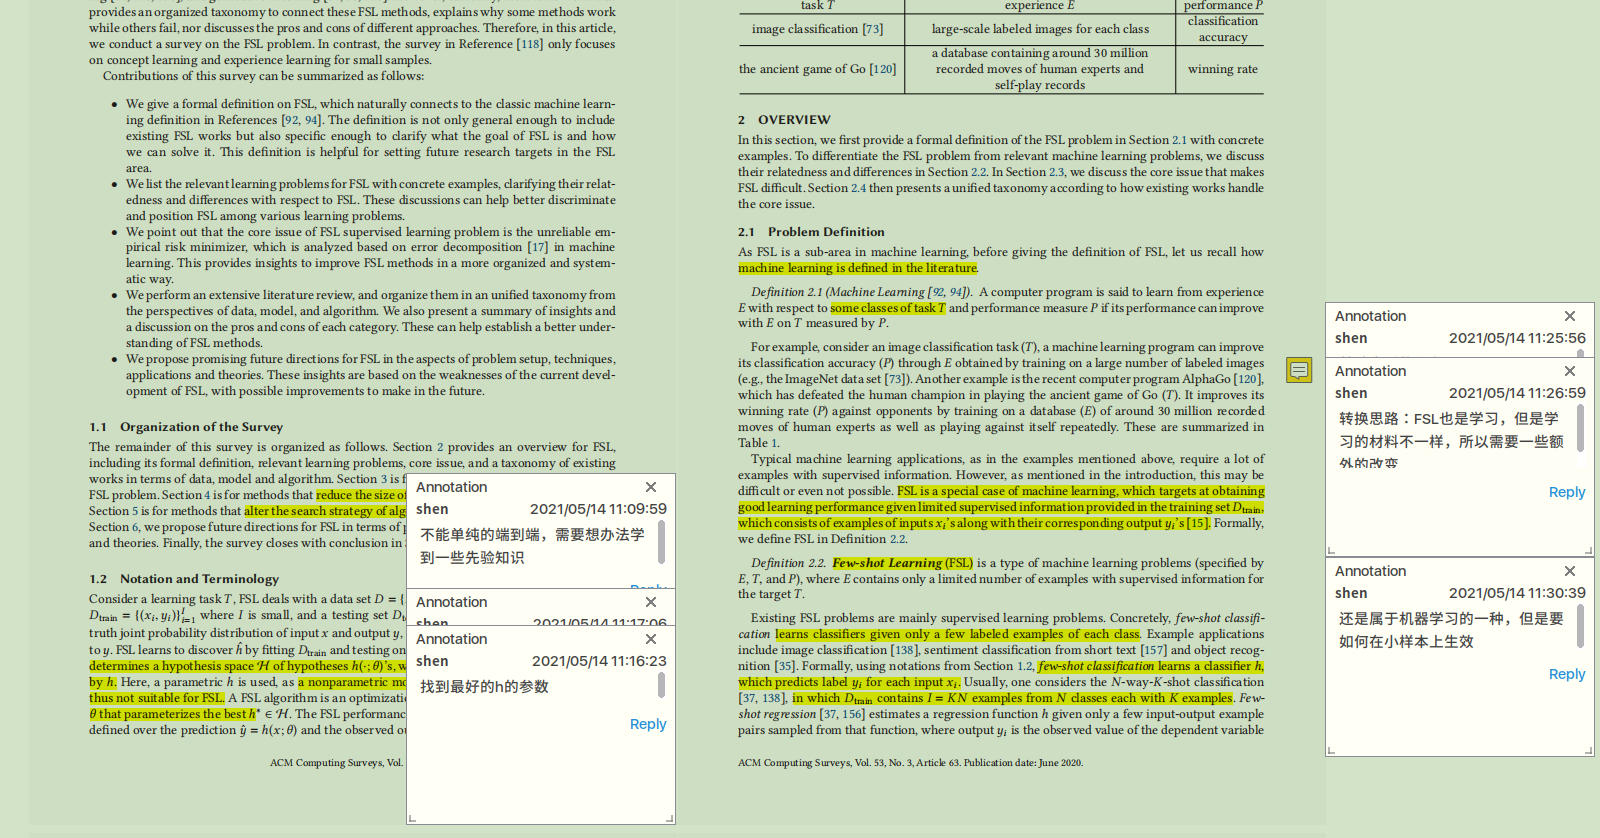
\includegraphics[width=1.1\textwidth]{figures/fsl.png}
                    \caption{FSL综述阅读}
                    \label{fig:fsl}
                \end{figure}

                \column{.26\textwidth}
                \begin{figure}
                    \centering
                    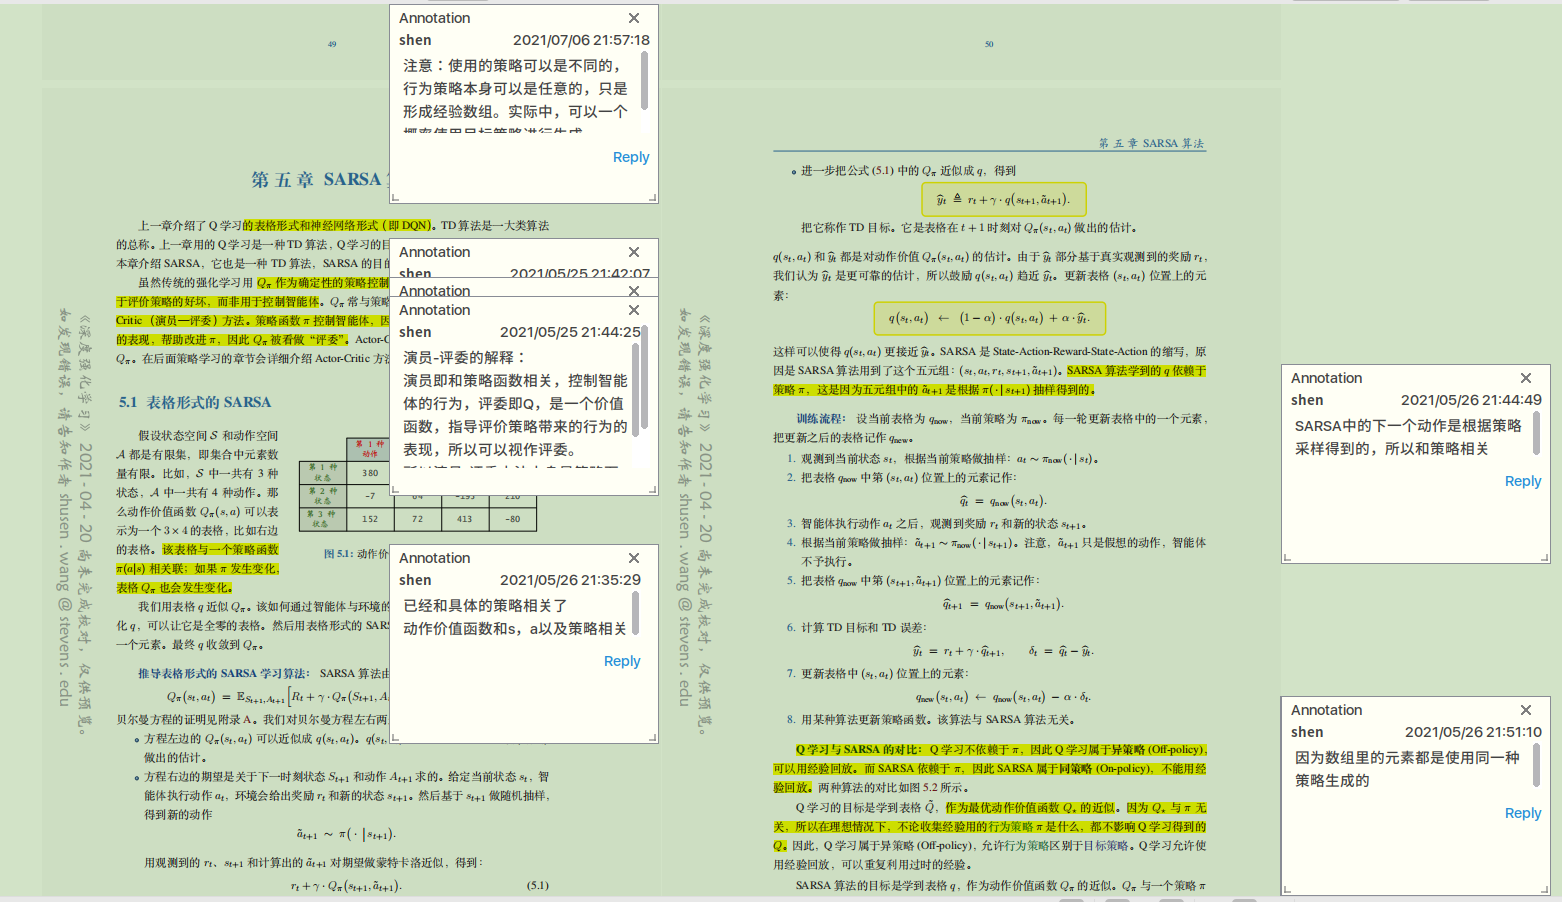
\includegraphics[width=1.1\textwidth]{figures/rl.png}
                    \caption{DeepRL书籍阅读}
                    \label{fig:rl}
                \end{figure}

                \column{.26\textwidth}
                \begin{figure}
                    \centering
                    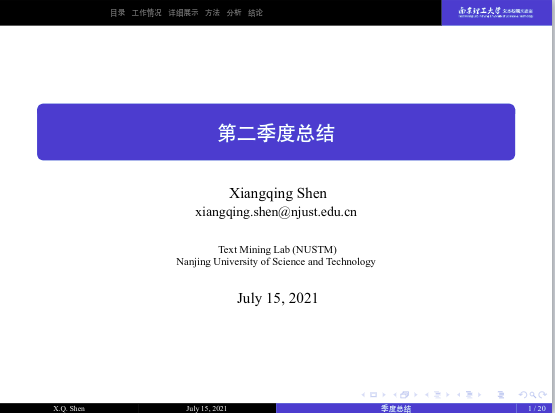
\includegraphics[width=1.1\textwidth]{figures/latex.png}
                    \caption{Beamer模版}
                    \label{fig:beamer}
                \end{figure}

            \end{columns}
            这段时间根据需要穿插完成了一些其他任务,如针对事件抽取任务阅读了一篇FSL的综述,系统学习了强化学习,\LaTeX 并改编了一个NUSTM主题的Beamer模版,系统学习了变分推断,完成了智能系统的课程作业。
		\end{frame}
		
        \begin{frame}
		  \frametitle{\textbf{CCKS2021数据收集(第7周)}}
			\begin{figure}[!t]
            \centering
            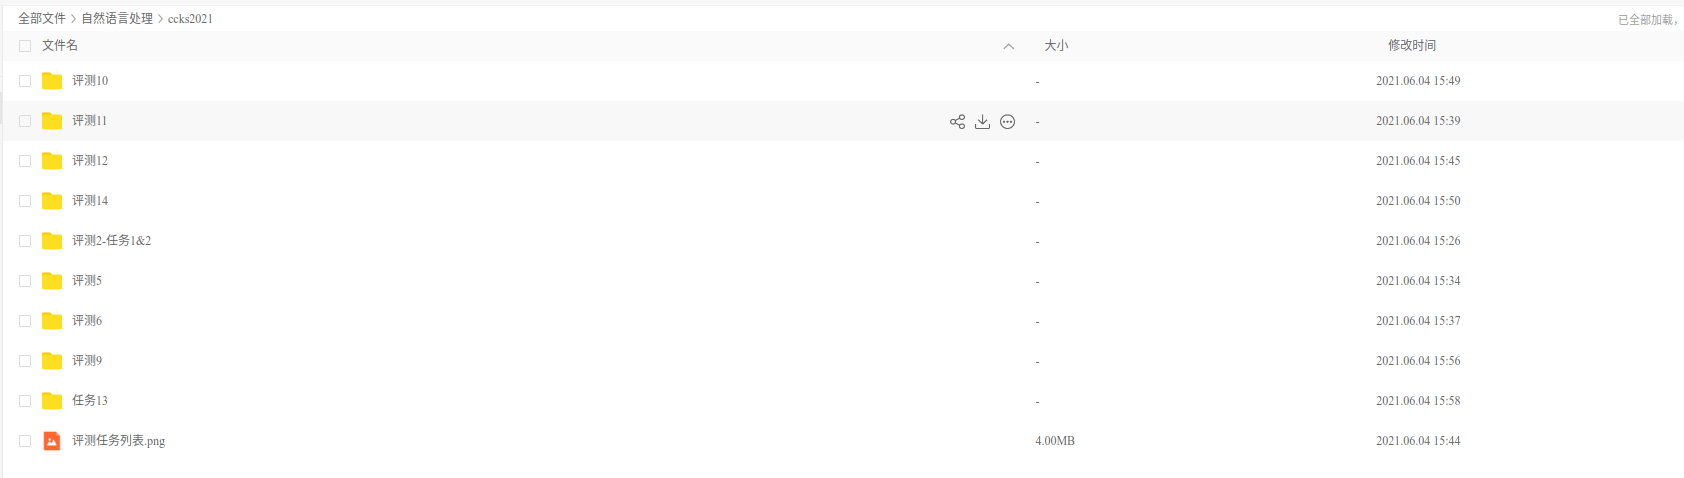
\includegraphics[width=4in]{figures/ccks.png}
            \caption{CCKS2021数据集收集}
            \label{fig:ccks}
            \end{figure}
            目前仅公布训练集、部分验证集,测试集没有公布,本月底预计全部公布,届时可以收集完毕。\\
            目前数据全部存放在百度网盘中。
		\end{frame}
		
        \begin{frame}
		  \frametitle{\textbf{事理图谱的调研和入门(第7-11周)}}
            \begin{block}{\textbf{工作内容}}
                \begin{itemize}
                    \item 大量阅读事理图谱论文:包括李忠阳的博士论文,小论文和相关重要的事理图谱相关的论文。
                    \item 维护了组内的事理图谱相关的论文列表。
                    \item 根据论文阅读过程中的需要复习了强化学习。
                    \item 完成了海量数据分析的课程作业。
                \end{itemize}
            \end{block}
		\end{frame}

        \begin{frame}
		  \frametitle{\textbf{AllenAI实验室工作跟进(第12-周)}}
            \begin{block}{\textbf{工作内容}}
                \begin{itemize}
                    \item 开始跟进AllenAI实验室的工作,目前阅读相关论文3篇
                \end{itemize}
            \end{block}
		\end{frame}
		
\section[积累]{科研积累}


		\begin{frame}
		  \frametitle{\textbf{周报展示}}
            \begin{columns}[b]

                \column{.26\textwidth}
                \begin{figure}
                    \centering
                    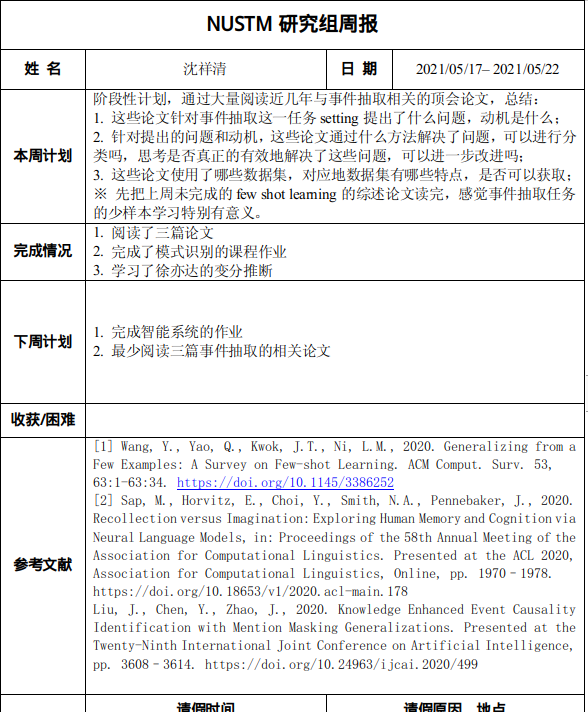
\includegraphics[width=1.1\textwidth]{figures/report1.png}
                    \caption{周报展示1}
                    \label{fig:report1}
                \end{figure}

                \column{.26\textwidth}
                \begin{figure}
                    \centering
                    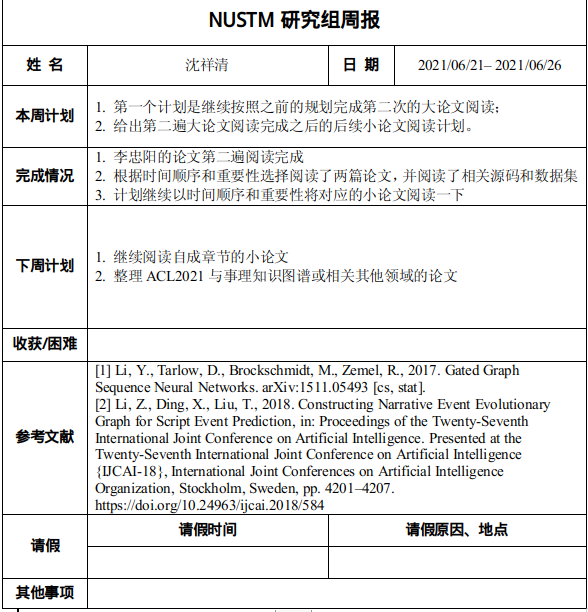
\includegraphics[width=1.1\textwidth]{figures/report2.png}
                    \caption{周报展示2}
                    \label{fig:report2}
                \end{figure}

                \column{.26\textwidth}
                \begin{figure}
                    \centering
                    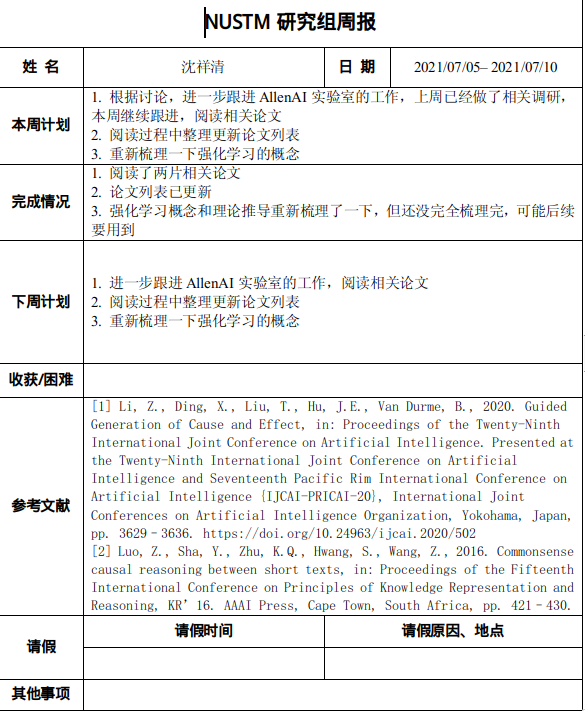
\includegraphics[width=1.0\textwidth]{figures/report3.png}
                    \caption{周报展示3}
                    \label{fig:report3}
                \end{figure}

            \end{columns}

		\end{frame}
		
		\begin{frame}
		  \frametitle{\textbf{本地文献管理}}
            \begin{figure}[!t]
            \centering
            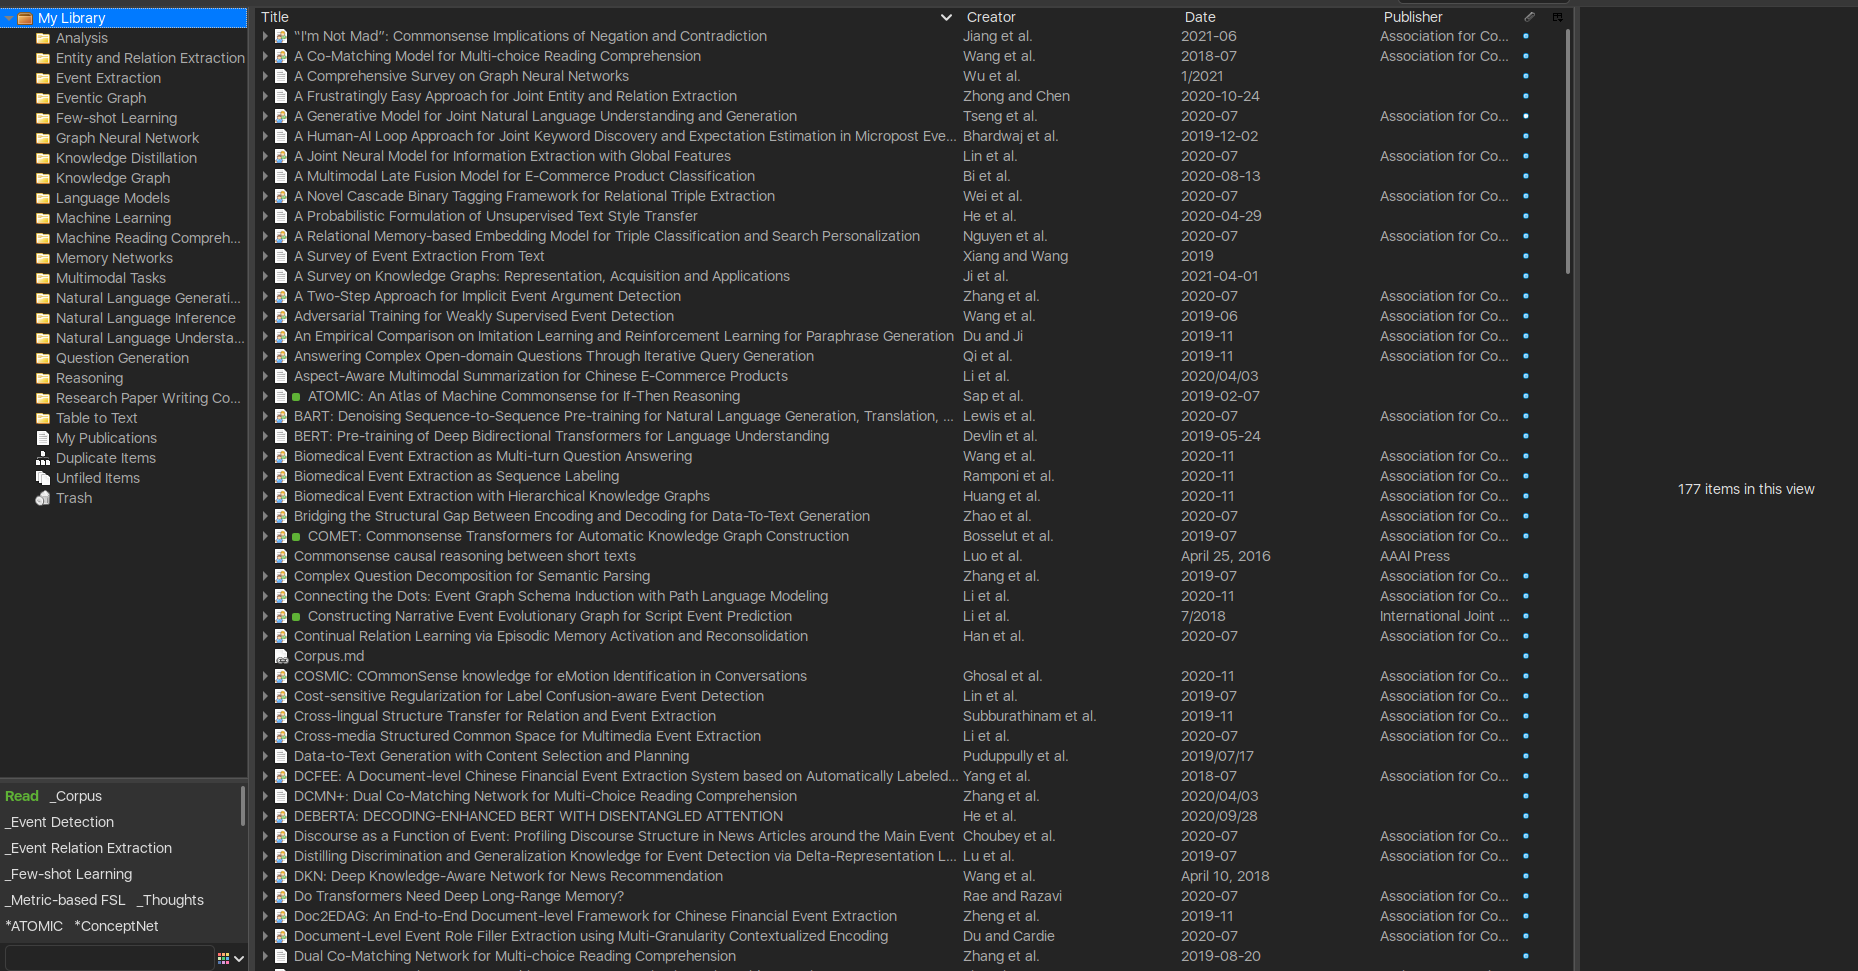
\includegraphics[width=4in]{figures/overview.png}
            \caption{本地文献管理概览}
            \label{fig:overview}
            \end{figure}
		\end{frame}
		
		\begin{frame}
		  \frametitle{\textbf{本地文献管理}}
            \begin{figure}[!t]
            \centering
            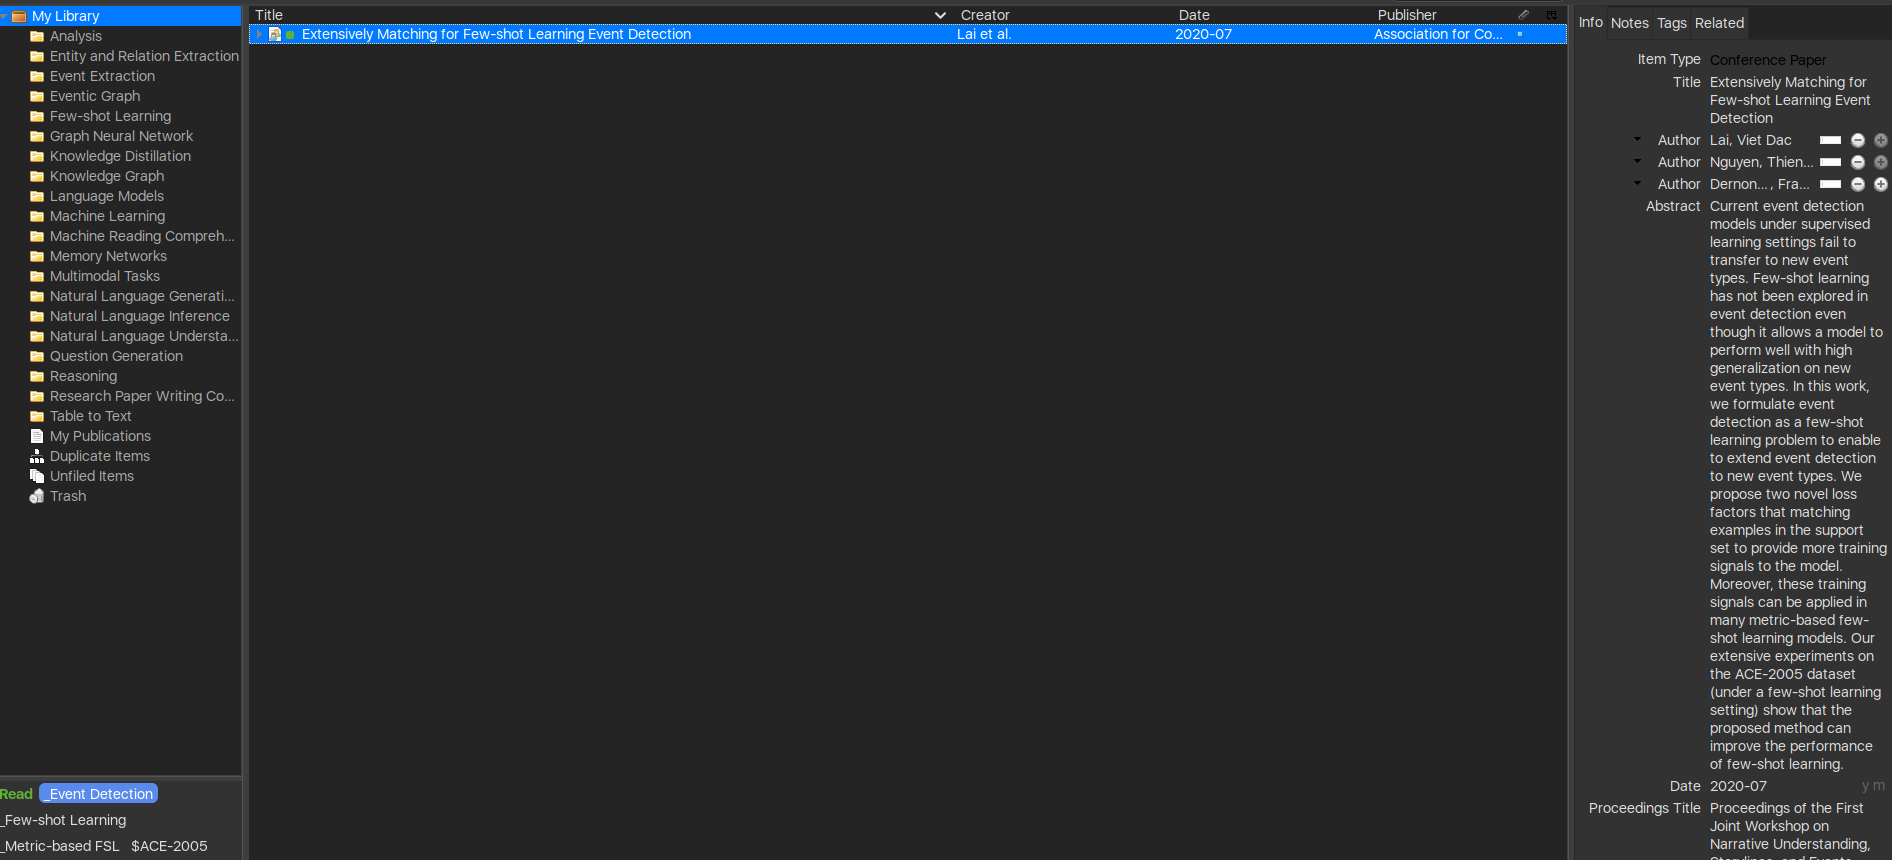
\includegraphics[width=4in]{figures/category.png}
            \caption{某种细分类别的文献}
            \label{fig:category}
            \end{figure}
		\end{frame}

		\begin{frame}
		  \frametitle{\textbf{本地文献管理}}
            \begin{figure}[!t]
            \centering
            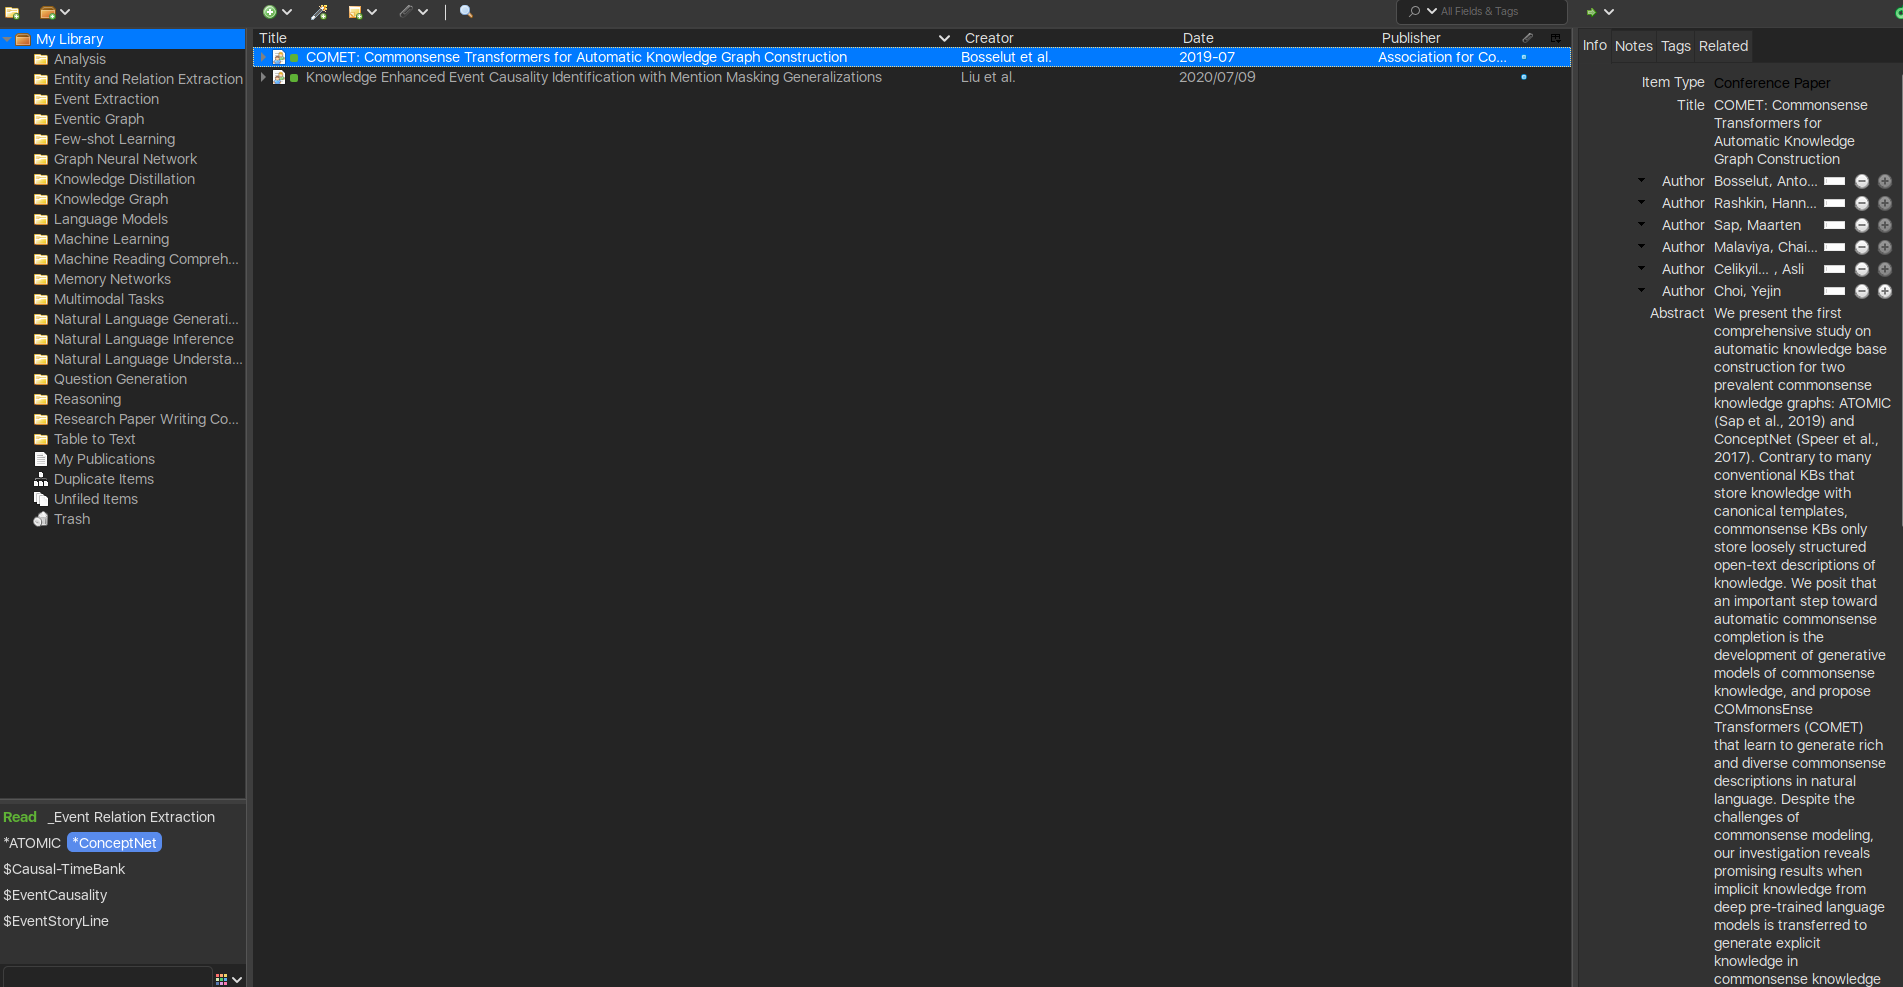
\includegraphics[width=4in]{figures/kg2.png}
            \caption{使用到某种知识图谱的文献}
            \label{fig:kg2}
            \end{figure}
		\end{frame}
		
		\begin{frame}
		  \frametitle{\textbf{本地文献管理}}
            \begin{figure}[!t]
            \centering
            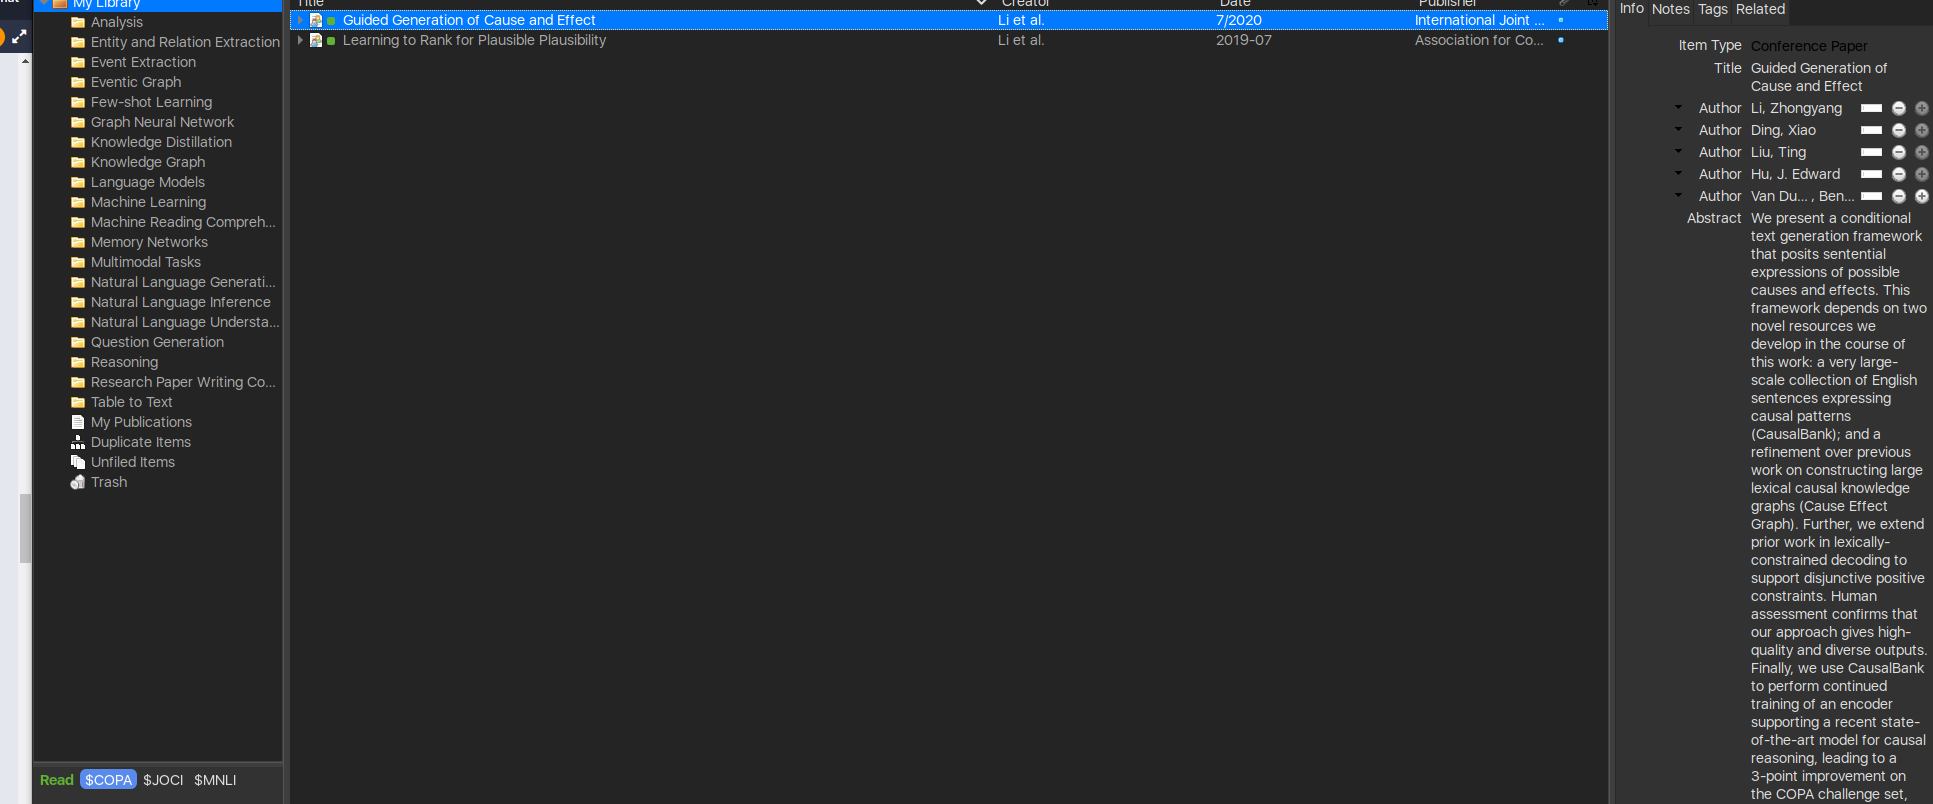
\includegraphics[width=4in]{figures/dataset.png}
            \caption{使用到某种数据集的文献}
            \label{fig:dataset}
            \end{figure}
		\end{frame}

		\begin{frame}
		  \frametitle{\textbf{本地文献管理}}
            \begin{figure}[!t]
            \centering
            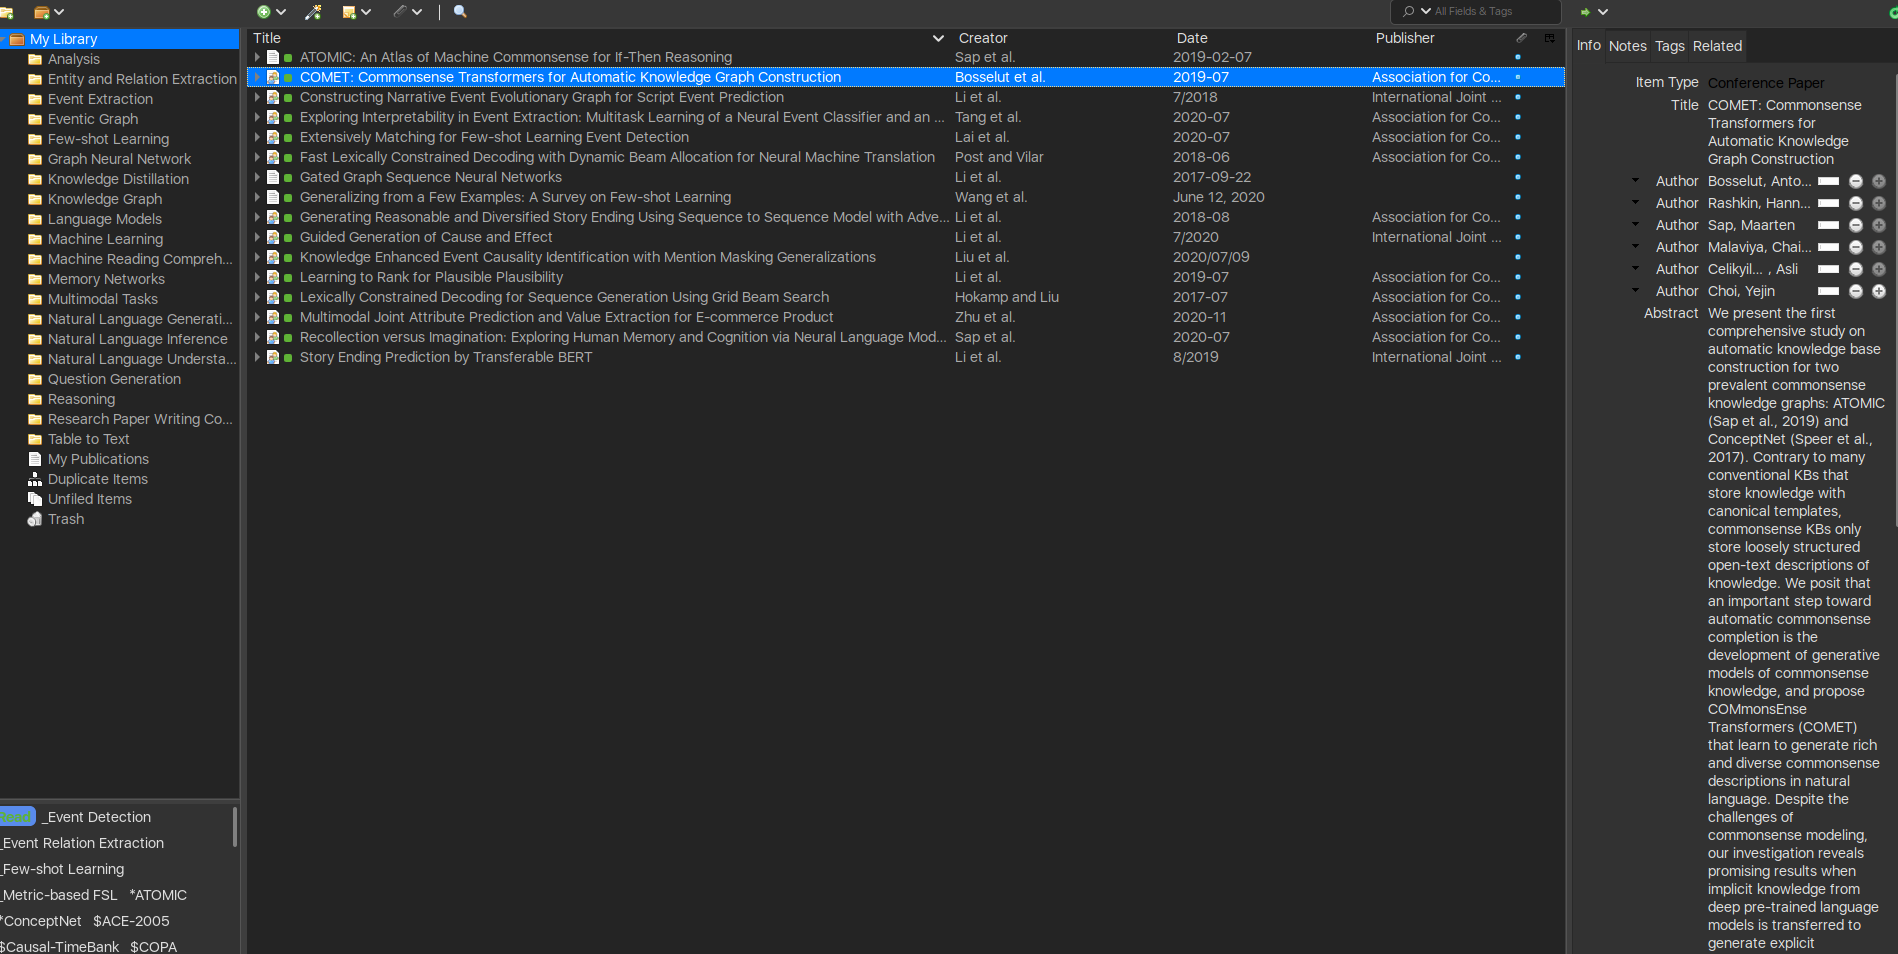
\includegraphics[width=4in]{figures/read.png}
            \caption{绿色标记已读文献}
            \label{fig:read}
            \end{figure}
		\end{frame}

		\begin{frame}
		  \frametitle{\textbf{组内阅读列表维护}}
            \begin{figure}[!t]
            \centering
            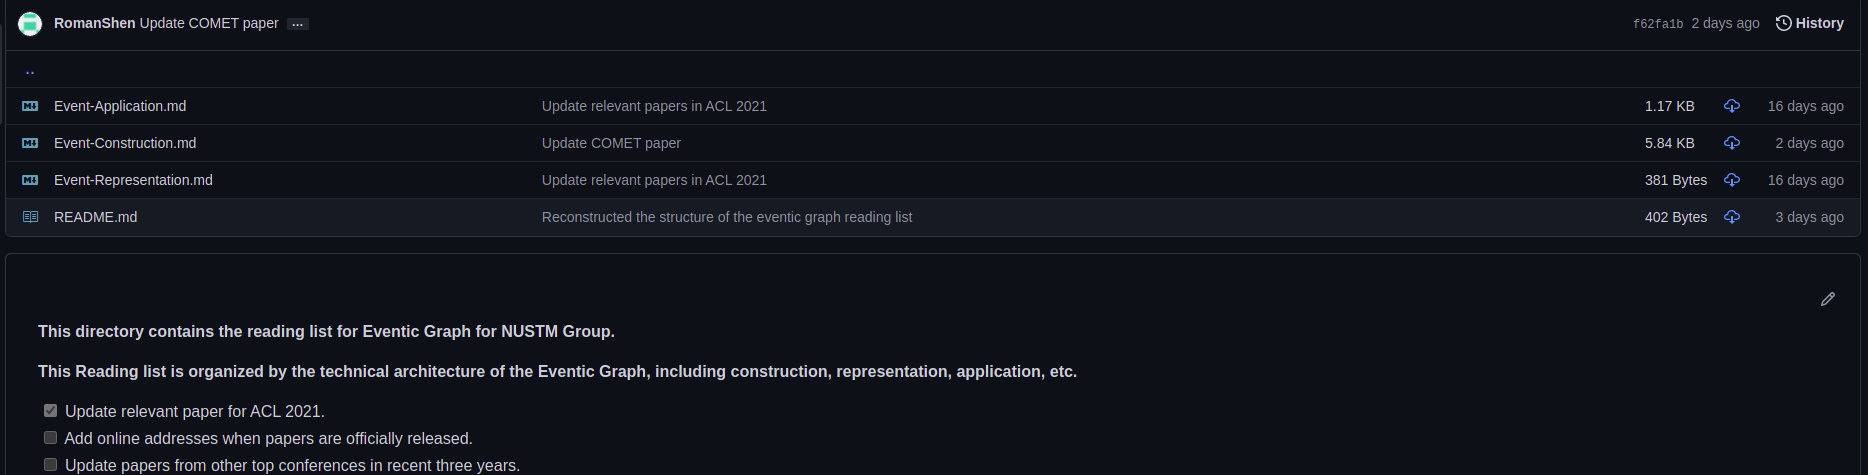
\includegraphics[width=4in]{figures/reading_list.png}
            \caption{事理图谱相关的论文列表}
            \label{fig:reading_list}
            \end{figure}
            目前主要分为三个部分:图谱的构建、表示和应用。构建部分涉及到的细分类别有事件抽取、事件检测、事件关系识别(因果)、图谱构建(ATOMIC)、图谱补全(COMET)等论文;表示部分包括事理图谱的节点和边的嵌入表示学习的论文;应用部分包括将事理图谱实际应用到某个任务上的论文。
		\end{frame}
		
        \begin{frame}
            \begin{columns}[b]
                \column{.45\textwidth}
                \begin{figure}
                    \centering
                    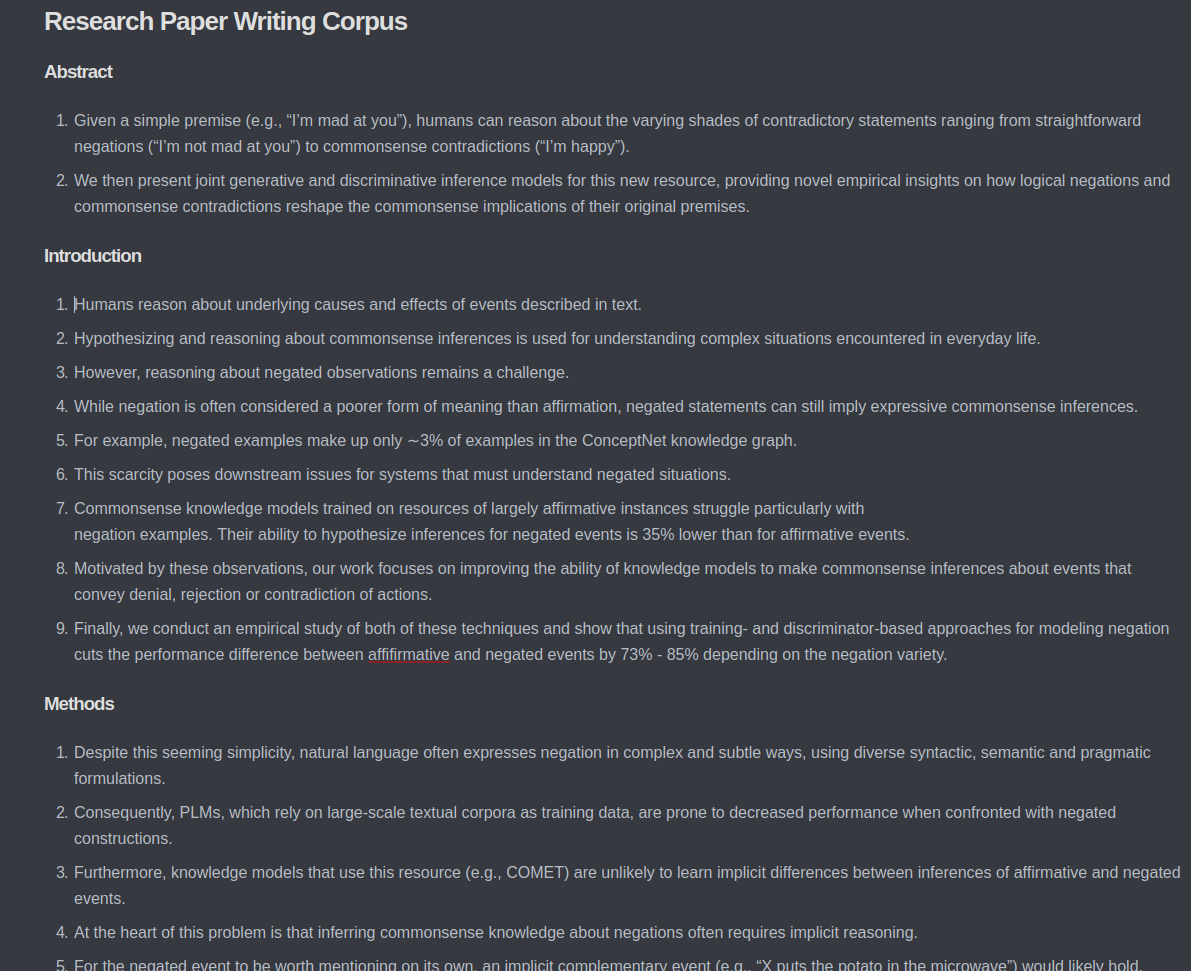
\includegraphics[width=1.1\textwidth]{figures/corpus.png}
                    \caption{写作素材积累}
                    \label{fig:corpus}
                \end{figure}

                \column{.45\textwidth}
                \begin{figure}
                    \centering
                    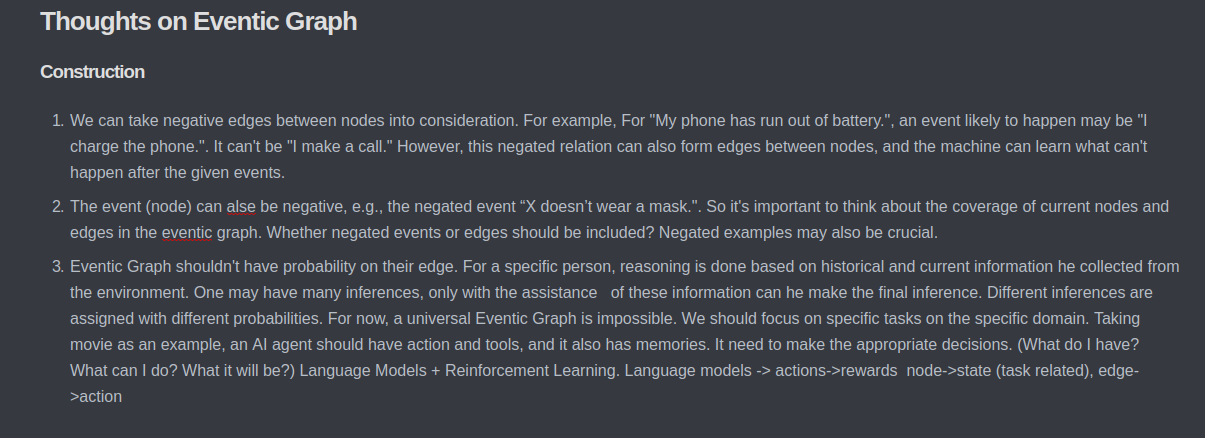
\includegraphics[width=1.1\textwidth]{figures/thoughts.png}
                    \caption{阅读文献过程中的一些想法记录}
                    \label{fig:thoughts}
                \end{figure}

            \end{columns}        
        \end{frame}

\section[计划]{下季度计划}


		\begin{frame}
		  \frametitle{\textbf{结论}}
		
		  \begin{itemize}
		    \item SMS生态系统在智能手机时代出现了新的发展,加入了更多新的设备和参与者。
		    \item 公共网关为用户提供了基于SMS的各种安全解决方案。
            \item 根据该研究,将SMS作为安全信道传递敏感信息存在一定的危险性。一些一次性的消息传递机制亟待改进\blfootnote{[1] Xiangqing Shen. Hello} \cite{Liao0ZNC18}。
            \item 至于短信滥用,公共网关可以用于规避一些安全性较差的认证机制,或进行PVA欺诈行为\cite{Liao0ZNC18}。
		  \end{itemize}
		\end{frame}
		
        \begin{frame}
            \frametitle{\textbf{总结}}
            \begin{block}{代表工作的总结}
                \begin{itemize}
                    \item 李忠阳的工作特点:聚焦于\textbf{某一特定领域}(交通、金融),以\textbf{高度抽象化的谓词短语作为事件节点}。根据特定领域的事件关联的特点,只关注于\textbf{某一具体事件关系}(如交通领域只关注时序关系,金融领域只关注因果关系),采用设计\textbf{模版}的方法在大规模语料上抽取相应的关系,经过抽象化后形成事理图谱。然后将构建好的事理图谱投入到相关领域的应用中。(具体->抽象->具体)
                    \item AllenAI的工作特点:不聚焦于特定领域,构建是通过\textbf{众包}。利用语言模型的强大能力,使用\textbf{有监督}的语料训练语言模型,使其可以在\textbf{预先设计好的事件关系}上推理接下来可能发生的事件。在他们的工作中,事件之间的关系不再局限于一种,有\textbf{多种复杂的关系}。
                \end{itemize}

            \end{block}
        \end{frame}
        
        \begin{frame}
            \frametitle{\textbf{问题和优势}}
            \begin{block}{李忠阳}
                \begin{itemize}
                    \item 优势:优势是确实\textbf{具有实际的应用效果}。由于李忠阳的工作聚焦于某一特定领域的特定关系,所以构建的复杂性大大降低。例如在金融领域,如果只考虑因果关系,经过高度抽象化以后,实际的事件节点数量确实能够一定程度上覆盖可能的金融事件。不仅图谱的构建复杂度降低,也有可能投入实际的应用。
                    \item 问题:由于是领域和关系限定的,\textbf{图谱的关系过于简单}。虽然满足了图谱的基本要求,但是关系十分单一,实际上在他所有的工作中图谱只存在一种关系。
                \end{itemize}
            \end{block}
        \end{frame}
        \begin{frame}
            \frametitle{\textbf{问题和优势}}
            \begin{block}{AllenAI}
                \begin{itemize}
                    \item \small {优势:优势是确实是\textbf{比较通用的事理图谱雏形}。其中存在的事件关系比较复杂,可以描述现实世界中复杂的事件关系。}
                    \item \small {问题:\textbf{节点的抽象程度不够}。并且,在他们的工作中还有Base Event的概念。这里的Base Event实际上是数据集构建过程中设计好的模版事件,这些\textbf{Base Event之间不会有边相连},这是不符合逻辑的。另外,由于ATOMIC这种知识图谱是通用型的,但是鉴于现实世界的复杂性,其实\textbf{很难对所有可能的事件有一个满意的覆盖度}。如一个Base Event后可能有上千个可能事件,但图谱只提供了不足10个。而且,这种图谱目前\textbf{很难有实际的应用},因为现实世界中的事件演化和具体的人的状态,周围环境,历史积累等相关的。如对于一个盲人而言,拿电视遥控器的下一个动作就不太可能是打开电视机,目前这种知识图谱还无法做到根据盲人这一条件降低某些后续事件的}
                \end{itemize}
            \end{block}
        \end{frame}        
        \begin{frame}
            \frametitle{\textbf{下季度计划}}
            \begin{itemize}
                \item 继续阅读近几年的事理图谱相关的论文。
                \item 针对目前阅读的文献思考如下问题:事理图谱的表示应该是什么样的(如节点的内容抽象化到什么程度;节点是否只能是表示事件的动宾短语;边上的信息是否只能是简单的事件关系;鉴于现实世界的复杂性,可能事理图谱目前模仿知识图谱的表达方式是不科学的,事理图谱的构建是客观的,应用是主观的,在特定条件下,可能某些图谱里的事件就不会发生了,这在传统知识图谱中是不可能出现的,事理图谱或许本身就应该是一个条件语言模型;),需要构建通用的还是领域的事理图谱。下游任务和事理图谱的结合需要进一步探索:目前有两种方向,一种是一定程度简化场景,构建领域特定的知识图谱(类似李忠阳);一种是思考下游任务和图谱融合的范式,类似BERT在下游任务上的微调,具体到一个任务上,这种通用的图谱是否要进行一些结构上的变化,然后在这一任务的语料上进行进一步的补全等操作。
                \item 回答这些问题需要更多的文献阅读和思考。暂时没有更细致详细的计划思路,可能需要和老师讨论。
            \end{itemize}
        \end{frame}
            
\section*{}
            \begin{frame}

                \begin{center}
                    \begin{minipage}{1\textwidth}
                        \setbeamercolor{mybox}{fg=white, bg=black!60!green}
                        \begin{beamercolorbox}[wd=0.70\textwidth, rounded=true, shadow=true]{mybox}
                        \LARGE \centering Thanks for Listening.
                        \end{beamercolorbox}
                    \end{minipage}
                \end{center}

                \begin{figure}[!t]
                    \centering
                    
\includegraphics[width=.8\textwidth]{source/nustm_contact.png}
                    \label{figure4_ad}
                \end{figure}
            \end{frame}
            
\begin{frame}[allowframebreaks]
    \frametitle{参考文献}
        \bibliographystyle{acl_natbib.bst}
        \bibliography{my_bib.bib}
        %  \printbibliography[heading=none]
   
\end{frame}


\end{document}
